%% Los cap'itulos inician con \chapter{T'itulo}, estos aparecen numerados y
%% se incluyen en el 'indice general.
%%
%% Recuerda que aqu'i ya puedes escribir acentos como: 'a, 'e, 'i, etc.
%% La letra n con tilde es: 'n.


\chapter{Resultados}


\section{Paquete de R \emph{geneticae}}

Siguiendo el flujo de trabajo descripto en el capítulo anterior fue posible desarrollar el paquete de R \emph{geneticae} que implementa los métodos estadísticos discutidos para el análisis de datos de EMA.

El paquete fue enviado a CRAN, donde pasó los exhaustivos controles de R CMD check exitosamente, logrando así una rápida aceptación. En el momento de la escritura de este informe, pasaron 3 semanas desde su publicación en el repositorio y cuenta con más de 400 descargas, a pesar de que aún no se ha hecho difusión del paquete. 

Para instalar la versión del paquete publicada en CRAN:  \textcolor{fandango}{install.packages(``geneticae")}, mientras que la versión en desarrollo se debe instalar desde el repositorio de GitHub:  \textcolor{fandango}{devtools::install\_github(``jangelini/geneticae")}. Una vez instalado el paquete, se debe cargar en la sesion de R mediante el comando: \textcolor{fandango}{library(geneticae)}. 

Información detallada sobre las funciones del paquete \emph{geneticae} se puede obtener mediante \textcolor{fandango}{help(package = ``geneticae")}. La ayuda para una función, por ejemplo \textcolor{fandango}{imputation()}, en una sesión R se puede obtener usando \textcolor{fandango}{?imputation} o \textcolor{fandango}{help(imputation)}. La función \textcolor{fandango}{browseVignettes(``geneticae")} permite obtener la viñeta del paquete, es decir una descripción el problema que está diseñado para resolver así como ejemplos de aplicación del mismo. 

Además, se encuentra disponible una página web\footnote{\url{https://jangelini.github.io/geneticae/}} que contiene una breve descripción de la utilidad del paquete, las funciones que se incluyen en él, un tutorial de uso, un enlace de acceso a la aplicación web Shiny, entre otros elementos.


\subsection{Conjuntos de datos en \emph{geneticae}}
\label{subsec:datosejemplos}
El paquete \emph{geneticae} proporciona dos conjuntos de datos que pueden utilizarse para ilustrar la metodología incluida para analizar los datos provenientes de EMA. 

\begin{itemize}[wide, nosep, labelindent = 0pt, topsep = 1ex, noitemsep,topsep=0pt]
\item \emph{yan.winterwheat dataset} \citep{Wright2020}: cuenta con información sobre el rendimiento de 18 variedades de trigo de invierno cultivadas en nueve ambientes en Ontario en 1993. A pesar de que el experimento contaba con cuatro bloques o réplicas en cada ambiente, sólo el rendimiento medio para cada combinación de variedad y ambiente se encuentra disponible.\\

\begin{tcolorbox}[skin=bicolor,
    colframe=aurometalsaurus,colback=backcolour,colbacklower=white,
    width=1\linewidth,
    height=0.24\linewidth,
    boxsep=-3mm]
\begin{lstlisting}[linewidth=\columnwidth]
data(yan.winterwheat)
head(yanwinterwheat)[1:3,]
\end{lstlisting}

\tcblower\vskip-\baselineskip
\tcblower
\vspace{0.5cm}
\footnotesize\begin{verbatim}
##   gen  env yield
## 1 Ann BH93 4.460
## 2 Ari BH93 4.417
## 3 Aug BH93 4.669
\end{verbatim}
\end{tcolorbox}

\item \emph{plrv dataset} \citep{deMendiburu2020}: contiene información sobre el rendimiento, el peso de planta y de la parcela de 28 genotipos en 6 localidades de Perú. Cada clon fue evaluado tres veces en cada ambiente. \\

\begin{tcolorbox}[skin=bicolor,
    colframe=aurometalsaurus,colback=backcolour,colbacklower=white,
    width=1\linewidth,
    height=0.24\linewidth,
    boxsep=-3mm]
\begin{lstlisting}
data(plrv)
head(plrv)[1:3,]
\end{lstlisting}

\tcblower\vskip-\baselineskip
\tcblower
\vspace{0.5cm}
\footnotesize\begin{verbatim}
##   Genotype Locality Rep WeightPlant WeightPlot    Yield
## 1   102.18     Ayac   1   0.5100000       5.10 18.88889
## 2   104.22     Ayac   1   0.3450000       2.76 12.77778
## 3   121.31     Ayac   1   0.5425000       4.34 20.09259
\end{verbatim}
\end{tcolorbox} 
\end{itemize}
   
  
\subsection{Uso del paquete para ajustar el modelo AMMI}

Para visualizar el efecto de IGA se utiliza el biplot GE obtenido del modelo AMMI a través de la función \textcolor{fandango}{rAMMI()}, que requiere datos en formato largo, es decir, cada fila corresponde a una observación y cada columna a una variable (genotipo, ambiente, fenotipo observado y, si existe, repetición). Si cada genotipo ha sido evaluado más de una vez en cada ambiente, la media fenotípica para cada combinación de genotipo y ambiente se calcula internamente y luego se estima el modelo. El conjunto de datos puede contener variables adicionales no utilizadas en el análisis (a diferencia de lo que ocurre con muchos softwares y funciones de R disponibles hasta el momento). No se permiten valores perdidos pero se pueden imputar como se indica en la subsección \ref{subsec:metimp}. 

El primer argumento de \textcolor{fandango}{rAMMI()} es el conjunto de datos de entrada, luego se indican los nombres de las columnas en las cuales se encuentra la información necesaria para aplicar la técnica y por último el biplot que se desea obtener que por defecto es el derivado del modelo AMMI clásico. Opcionalmente, se puede agregar el porcentaje de IGA explicado por el biplot como una nota al pie mediante el argumento \emph{footnote = T} y un título con \emph{titles = T}. 

El biplot clásico para el conjunto de datos \emph{yan.winterwheat} se muestra en la figura
\ref{fig:ammibip}. En este ejemplo BH93, KE93 y OA93 son los ambientes que más contribuyen a la interacción ya que sus vectores son los de mayor magnitud. Los cultivares m12 y Kat presentan patrones de interacción similares (sus identificadores están próximos entre sí) y son muy diferentes de Ann y Aug, por ejemplo. La cercanía entre el cultivar Dia y el ambiente BH93 indica una fuerte asociación positiva entre ellos, lo que significa que BH93 es un ambiente extremadamente favorable para ese genotipo. Como los marcadores OA93 y Luc son opuestos, este ambiente es considerablemente desfavorable para ese genotipo. Por último, Cas y Reb están cerca del origen, lo que significa que se adaptan en igual medida a todos los ambientes.

\begin{tcolorbox}[skin=bicolor,
    colframe=aurometalsaurus,colback=backcolour,colbacklower=white,
    width=1\linewidth,
    height=0.82\linewidth,
    boxsep=-3mm]
\begin{lstlisting}
rAMMI(yan.winterwheat, genotype = ``gen", environment = ``env", 
      response = ``yield", type = ``AMMI", footnote = F, titles = F)
\end{lstlisting}
\tcblower\vskip-\baselineskip
\tcblower
\begin{figure}[H]
	\begin{center}
		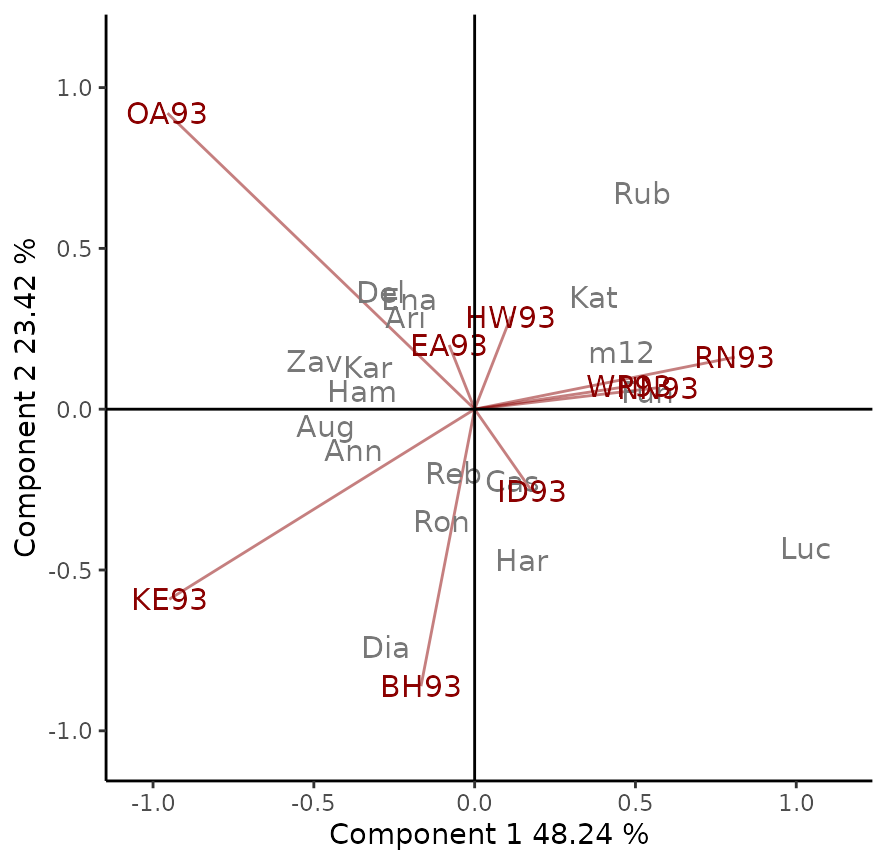
\includegraphics[width=0.50\textwidth]{./Graficos/AMMI_biplot.png}
	\end{center}
	\caption{Biplot GE obtenido del modelo AMMI clásico basado en los datos de rendimiento de trigo de invierno obtenidos en Ontario en 1993. El 71,66\% de la variabilidad de la IGA se explica por los dos primeros términos multiplicativos. Los cultivares se muestran en letras minúsculas y los ambientes en mayúsculas. }
	\label{fig:ammibip}
\end{figure}
\end{tcolorbox}


Como se mencionó anteriormente, el modelo AMMI, en su forma estándar, asume que no hay valores atípicos en los datos. Por lo tanto, en presencia de \emph{outliers} se debe utilizar alguna de las alternativas robustas propuestas por \citet{Rodriguesetal2016}, las cuales no se encuentran disponibles en R hasta el momento. Sin embargo, dada la importancia práctica de este reciente avance metodológico, se incluyeron en la función \textcolor{fandango}{rAMMI()}. Para obtener los biplots GE derivados de los modelos robustos se debe indicar en el argumento \emph{type} cuál de ellos se desea ajustar: ``rAMMI", ``hAMMI", ``gAMMI", ``lAMMI" o ``ppAMMI".

Dado que el conjunto de datos de muestra \emph{yan.winterwheat} no presenta valores atípicos, las conclusiones obtenidas con biplots robustos no difieren de las obtenidas con el biplot clásico \citep{Rodriguesetal2016}. Por lo tanto, no se presenta ninguna interpretación de los biplots robustos. 


\subsection{Uso del paquete para ajustar el modelo SREG}
\label{subsec:SREGpaquete}
Con el fin de visualizar conjuntamente el efecto de G e IGA \citet{Yanetal2000} propuso el biplot GGE mediante el cual se pueden abordar diversos aspectos relacionados con la evaluación de genotipos y ambientes. Para obtener dicho biplot en primer lugar se debe ajustar el modelo SREG mediante \textcolor{fandango}{GGEmodel()} que, del mismo modo que \textcolor{fandango}{rAMMI()}, requiere datos en formato largo. Si bien esta función invoca a \textcolor{fandango}{GGEModel()} del paquete \emph{GGEBiplots} \citep{Dumble2017}, al ser utilizada mediante \emph{geneticae} se permiten repeticiones y variables adicionales en el conjunto de datos. El rasgo fenotípico para cada combinación de genotipo y ambiente debe estar registrado, sino se debe recurrir previamente a alguna técnica de imputación para completar los datos (subsección \ref{subsec:metimp}). 

Se presenta a continuación la sentencia utilizada para ajustar el modelo SREG para el conjunto de datos \emph{yan.winterwheat}.

\begin{center}
\begin{tcolorbox}[colframe=aurometalsaurus,colback=backcolour,colbacklower=white,
   				width=1\linewidth,
    			height=0.08\linewidth,
    			boxsep=-3mm]
\begin{lstlisting}
GGE1 <- GGEmodel(yan.winterwheat, genotype = ``gen", environment = ``env",  response = ``yield", rep = NULL,  centering = ``tester", scaling = ``none",  SVP = ``symmetrical")
\end{lstlisting}
\end{tcolorbox}
\end{center}

El primer argumento es el nombre del conjunto de datos y en los siguientes se indican los nombres de las columnas que contienen la información de los genotipos, ambientes y del rasgo fenotípico de interés. Por defecto, la función considera que no hay réplicas en el conjunto de datos, sin embargo, si existieran en el parámetro \emph{rep} se debe indicar el nombre de la columna con dicha información. Otros argumentos son el método de centrado, de partición de los valores singulares (SVP por sus siglas en inglés, \emph{Singular Value Partition}) y escalado. Por defecto los datos se centran utilizando la opción \emph{centering=``tester"} lo cual resulta en el modelo SREG. La elección del método de SVP no altera las relaciones o interacciones relativas entre los genotipos y los ambientes, aunque la apariencia del biplot será diferente \citep{Yan2002}. El método de partición de los valores singulares centrado en los genotipos (\emph{SVP=``row"}) muestra la interrelación entre genotipos con mayor precisión, el enfocado a los ambientes (\emph{SVP=``column"}) es el más informativo de las interrelaciones entre los ambientes, mientras que el simétrico (\emph{SVP=``symmetrical"}) permite visualizar la magnitud relativa tanto de la variación de los genotipos como de los ambientes, por lo que se utiliza por defecto. Por último, se indica que los datos no se deben escalar con el parámetro \emph{scaling=``none"}. 

La salida de \textcolor{fandango}{GGEModel()} es una lista con los siguientes objetos:
\begin{itemize}
\item \emph{coordgenotype}: coordenadas para los genotipos en cada componente.
\item \emph{coordenviroment}: coordenadas para los ambientes en cada componente.
\item \emph{eigenvalues}: vector de autovalores para cada componente.
\item \emph{vartotal}: variancia general.
\item \emph{varexpl}: porcentaje de varianza explicado por cada componente.
\item \emph{labelgen}: nombres de los genotipos.
\item \emph{labelenv}: nombres de los ambientes.
\item \emph{axes}: etiquetas de los ejes.
\item \emph{Data}: datos escalados y centrados.
\item \emph{centering}: método de centrado.
\item \emph{scaling}: método de escala.
\item \emph{SVP}: método de partición. 
\end{itemize}


Utilizando la salida de \textcolor{fandango}{GGEmodel()}, la función 
\textcolor{fandango}{GGEPlot()} crea numerosas vistas del biplot GGE que permiten dar respuesta a distintos objetivos de los fitomejoradores. En estos gráficos los cultivares se muestran en minúsculas y los ambientes en mayúsculas. El método de centrado, escalado y SVP se muestran en una nota al pie junto con el porcentaje de G e IGA explicado por los dos ejes al agregar el argumento \emph{footnote = T} y un título con \emph{titles = T}. \\

\textbf{Comparaciones simples utilizando GGE biplot}

El biplot básico se obtiene con el parámetro \emph{type = ``Biplot"} (Figura \ref{fig:ggebip}). En este ejemplo, el 78\% de la variabilidad de G e IGA se explica por los dos primeros términos multiplicativos. Los ángulos entre los marcadores de genotipos y entre los vectores ambientales son utilizados para interpretar el gráfico. Así, por ejemplo, Kat tiene un rendimiento por debajo de la media en todos los ambientes debido a su ángulo superior a $90^{\circ}$ con todos ellos. Por otro lado, Fun presenta un rendimiento superior a la media en todas las localidades excepto OA93 y KE93, como lo indican los ángulos agudos. La longitud de los vectores ambientales es una medida de la capacidad del ambiente para discriminar entre cultivos. 


\begin{tcolorbox}[skin=bicolor,
    colframe=aurometalsaurus,colback=backcolour,colbacklower=white,
    width=1\linewidth,
    height=0.82\linewidth,
    boxsep=-3mm]
\begin{lstlisting}
GGEPlot(GGE1, type = ``Biplot", footnote = F, titles = F)
\end{lstlisting}
\tcblower\vskip-\baselineskip
\tcblower
\begin{figure}[H]
	\begin{center}
		\includegraphics[width=0.50\textwidth]{./Graficos/GGE_biplot.png}
	\end{center}
	\caption{Biplot GGE basado en datos de rendimiento de trigo de invierno obtenido de Ontario en 1993. El método de partición de valores singulares utilizado es el simétrico (opción por defecto). El 78\% de la variabilidad de G e IGA se explica por los dos primeros términos multiplicativos. Los cultivares se muestran en minúsculas y los entornos en mayúsculas. }
	\label{fig:ggebip}
\end{figure}
\end{tcolorbox} 


Con frecuencia, los mejoradores necesitan identificar los cultivares más adaptados a un ambiente particular, por ejemplo OA93. Para esto \citep{YanKang2003} sugieren construir un eje del ambiente de interés (OA93), trazando una recta que una el identificador del ambiente y el origen de coordenadas, y lo denominan eje OA93. Los genotipos se  clasifican en función del rendimiento en dicho ambiente de acuerdo con sus proyecciones, en la dirección indicada por el eje OA93 (Figura \ref{fig:selectEyG} (A)). Para obtener esta vista del biplot GGE, se indica la opción \emph{Selected Environment} en el argumento \emph{type} de la función y el ambiente a evaluar en el argumento  \emph{selectedE}. En este ejemplo, el cultivar de mayor rendimiento fue es Zav seguido por Aug, Ham hasta llegar al genotipo Luc, que es el de menor rendimiento en ese ambiente. El eje perpendicular al del ambiente de interés separa los genotipos con rendimiento mayor al promedio: de Zav a Cas, de aquellos con valores inferior a la media, de Ema a Luc, en OA93.
 
En forma similar, es posible determinar el ambiente más adecuado para un cultivar graficando una línea que conecte el origen de coordenadas y el marcador del genotipo de interés, por ejemplo Kat, como se muestra en la figura \ref{fig:selectEyG} (B) \citep{YanKang2003}. Los ambientes se clasifican a lo largo del eje del genotipo en la dirección indicada por la flecha. Para obtener este gráfico la opción  \emph{Selected Genotype} debe indicarse en el argumento \emph{type} y el genotipo de interés en \emph{selectedG}. El eje perpendicular al del genotipo separa los ambientes en los que el cultivar presentó un rendimiento por debajo y por encima del promedio. En este ejemplo, Kat presentó un desempeño por debajo de la media en todos los ambientes estudiados. \\

\begin{tcolorbox}[skin=bicolor,
    colframe=aurometalsaurus,colback=backcolour,colbacklower=white,
    width=1\linewidth,
    height=0.91\linewidth,
    boxsep=-3mm]
\begin{lstlisting}
# Ranking de cultivares en el ambiente OA93
GGEPlot(GGE1, type = ``Selected Environment", selectedE = ``OA93", footnote = F, titles = F)

# Ranking de ambientes para cultivar Kat
GGEPlot(GGE1, type = ``Selected Genotype", selectedG = ``Kat", footnote = F, titles = F)
\end{lstlisting}
\tcblower\vskip-\baselineskip
\tcblower
\begin{figure}[H]
	\begin{center}
		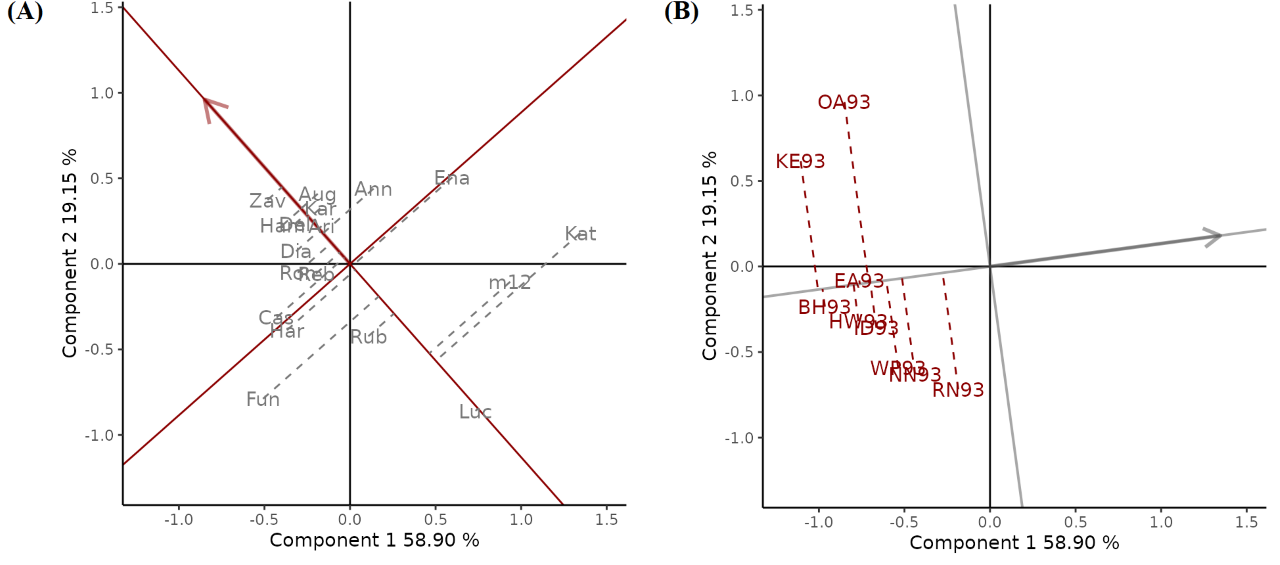
\includegraphics[width=0.95\textwidth]{./Graficos/SelectedGyE3.png}
	\end{center}
	\caption{ Ranking de (A) cultivares en el ambiente OA93 y (B) ambientes para cultivar Kat, basado en datos de rendimiento de trigo de invierno obtenido de Ontario en 1993. El método de partición de valores singulares utilizado es el simétrico (opción por defecto). El 78\% de la variabilidad de G e IGA se explica por los dos primeros términos multiplicativos. Los cultivares se muestran en minúsculas y los entornos en mayúsculas.}
	\label{fig:selectEyG}
\end{figure}
\end{tcolorbox} 


También es posible comparar dos cultivares, por ejemplo Kat y Cas, vinculándolos con una línea y trazando una recta perpendicular a ella (figura \ref{fig:comp2G}). Este biplot se obtiene con \emph{Comparison of Genotype} en el argumento \emph{type} y los genotipos a comparar en \emph{selectedG1} y \emph{selectedG2}. Cas fue más rendidor que Kat en todos los ambientes, ya que todos se ubican en el mismo lado de la línea perpendicular que Cas. \\

\begin{tcolorbox}[skin=bicolor,
    colframe=aurometalsaurus,colback=backcolour,colbacklower=white,
    width=1\linewidth,
    height=0.82\linewidth,
    boxsep=-3mm]
\begin{lstlisting}
GGEPlot(GGE1, type = ``Comparison of Genotype", selectedG1 = ``Kat", selectedG2 = ``Cas", footnote = F, titles = F)
\end{lstlisting}
\tcblower\vskip-\baselineskip
\tcblower
\begin{figure}[H]
	\begin{center}
		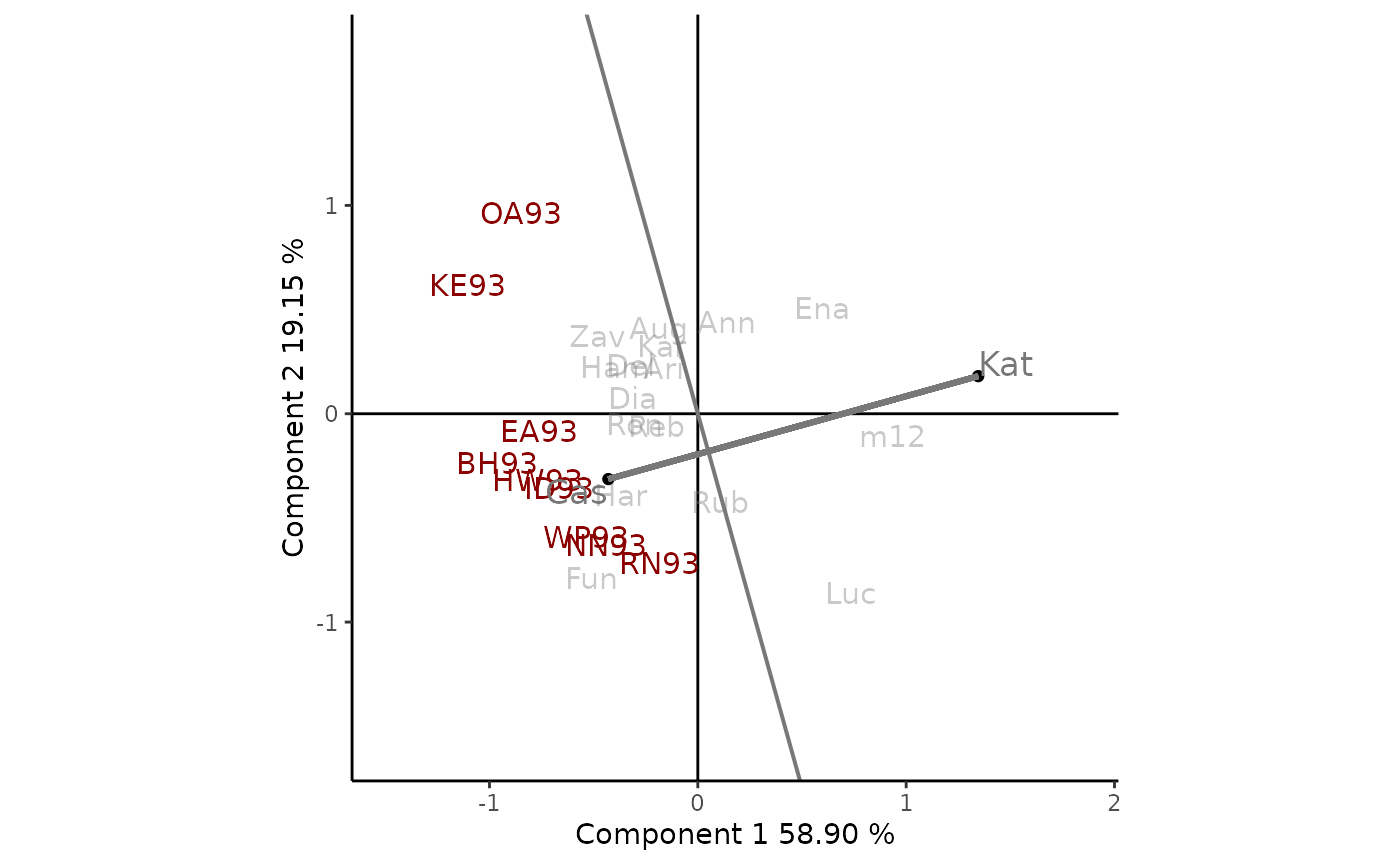
\includegraphics[width=0.50\textwidth]{./Graficos/GGE_comparisonG1yG2.png}
	\end{center}
	\caption{comparación de los cultivares Kat y Cas. El método de partición de valores singulares utilizado es el simétrico (opción por defecto). El 78\% de la variabilidad de G e IGA se explica por los dos primeros términos multiplicativos. Los cultivares se muestran en minúsculas y los entornos en mayúsculas. }
	\label{fig:comp2G}
\end{figure}
\end{tcolorbox}


\textbf{Identificación de mega-ambientes con GGE biplot}

La vista poligonal del biplot GGE, obtenida al indicar \emph{Which Won Where/What} en el argumento \emph{type}, proporciona un medio eficaz de visualización del patrón ``quíen ganó dónde"  de un conjunto de datos provenientes de EMA (Figura \ref{fig:poligono}).  El polígono se obtiene uniendo los cultivares (fun, zav, ena, kat y luc) que se encuentran más alejados del origen de coordenadas, de modo que todos los restantes se encuentren contenidos en el polígono. La distancia de los cultivares respecto del origen de coordenadas, en sus respectivas direcciones, es una medida de la capacidad de respuesta a los ambientes. Aquellos ubicados en los vértices son los más alejados, por lo tanto son los cultivares que más responden, mientras que los que se encuentran en el origen de coordenadas no responden en absoluto a los ambientes estudiados.

Las rectas perpendiculares a los lados del polígono dividen al biplot en mega-ambientes. El cultivar de mayor rendimiento en todos los ambientes de un mega-ambiente es el que se encuentra en el vértice del polígono. Por un lado, se observa que OA93 y KE93 conforman un mega-ambiente y que Zav es el mejor cultivar. El resto de los ambientes, forman otro mega-ambiente (identificado como ME1) siendo Fun el cultivar que se encuentra en el vértice. En el sector con ena, kat y luc en los vértices del polígono no se observó ningún ambiente, lo cual indica que estos cultivares fueron los menos rendidores en algunos o todos los ambientes considerados.\\

\begin{tcolorbox}[skin=bicolor,
    colframe=aurometalsaurus,colback=backcolour,colbacklower=white,
    width=1\linewidth,
    height=0.82\linewidth,
    boxsep=-3mm]
\begin{lstlisting}
GGEPlot(GGE1, type = ``Which Won Where/What", footnote = F, titles = F)
\end{lstlisting}
\tcblower\vskip-\baselineskip
\tcblower
\begin{figure}[H]
	\begin{center}
		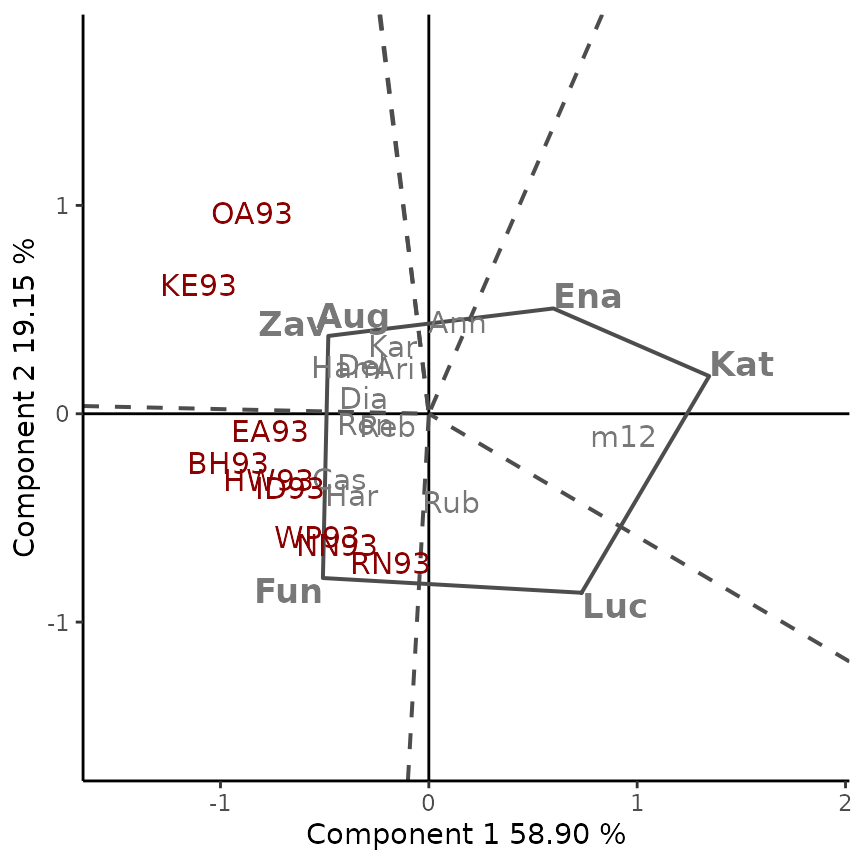
\includegraphics[width=0.48\textwidth]{./Graficos/GGE_whichwonwhere.png}
	\end{center}
	\caption{Vista poligonal del biplot GGE, que muestra qué cultivares presentaron mayor rendimiento en cada mega-ambiente. El método de partición de valores singulares utilizado es el simétrico (opción por defecto). El 78\% de la variabilidad de G e IGA se explica por los dos primeros términos multiplicativos. Los cultivares se muestran en minúsculas y los entornos en mayúsculas.}
	\label{fig:poligono}
\end{figure}
\end{tcolorbox}


\textbf{Evaluación de los cultivares dentro de un mega-ambientes con GGE biplot}

Una vez identificado los mega-ambientes, el siguiente paso es seleccionar cultivares dentro de cada uno de ellos. De acuerdo con la figura  \ref{fig:poligono}, zav es el mejor cultivar para los ambientes en uno de los mega-ambiente y fun para el otro. Sin embargo, los fitomejoradores generalmente no seleccionan un único cultivar en cada mega-ambiente, sino que evalúan a todos con el fin de conocer su desempeño (rendimiento y estabilidad).  

El biplot GGE, particularmente utilizando el factor de partición de la descomposición en valores singulares enfocando en los genotipos, es decir utilizando el argumento \emph{SVP=``row"} en la función \textcolor{fandango}{GGEmodel()}, proporciona un medio superior para visualizar tanto el rendimiento medio como la estabilidad de los genotipos. Esto se debe a que la unidad de ambos ejes para los genotipos es la unidad original de los datos. Además, dado que el interés radica en los genotipos y no en los ambientes, estos son omitidos del gráfico con el argumento \emph{sizeEnv = 0}.

La visualización del rendimiento medio y la estabilidad de los genotipos se logra dibujando una coordenada ambiental promedio (AEC, por sus siglas en inglés \emph{Average environment coordination}). Por ejemplo, la Figura \ref{fig:evaluacionG} (A)  muestra el AEC para el mega-ambiente ME1 compuesto por los entornos BH93, EA93, HW93, ID93, NN93, RN93 y WP93. La abscisa representa el efecto de G y la ordenada el de la IGA, que es una medida de la variabilidad o inestabilidad asociada con cada genotipo. Los cultivares se clasifican de acuerdo a su rendimiento medio a lo largo de la abscisa del AEC de acuerdo a la dirección de dicho eje, mientras que una proyección sobre la ordenada AEC muy alejada del origen, independientemente de la dirección, significa mayor inestabilidad. El cultivar de mayor rendimiento promedio en este mega-ambiente fue Fun, seguido por Cas y Har, mientras que Kat fue el de peor rendimiento medio. Rub y Dia son más variables y menos estables que otros cultivares, por el contrario, Cas, Zav, Reb, Del, Ari y Kar, fueron más estables. 

La Figura \ref{fig:evaluacionG} (B) compara los cultivares con uno considerado ``ideal” por ser el más rendidor y con estabilidad absoluta. Este cultivar ideal se usa como referencia, ya que rara vez existe. La distancia entre los cultivares y el ideal se puede utilizar como medida de conveniencia. Los círculos concéntricos ayudan a visualizar estas distancias. En el ejemplo, para el ME1, Fun es el más cercano al cultivo ideal, y por tanto el más deseable, seguido de Cas y Har, y Kat fue el más lejano. \\


\begin{tcolorbox}[skin=bicolor,
    colframe=aurometalsaurus,colback=backcolour,colbacklower=white,
    width=1\linewidth,
    height=1.05\linewidth,
    boxsep=-3mm]

\begin{lstlisting}

ME1 <- yan.winterwheat[yan.winterwheat(*@\$@*)env %in% c(``BH93", ``EA93",``HW93", ``ID93",``NN93", ``RN93", ``WP93"), ]
                                                   
# Modelo SREG enfocando SVD en los genotipos
GGE_Gpartition <- GGEmodel(ME1, genotype = ``gen", environment = ``env", response = ``yield", SVP = ``row")

# Visualizacion del rendimiento medio y la estabilidad
GGEPlot(GGE_Gpartition, type = ``Mean vs. Stability", footnote = F, titles = F, sizeEnv = 0)

# Ranking de los genotipos respecto a uno ideal
GGEPlot(GGE_Gpartition, type = ``Ranking Genotypes", footnote = F, titles = F, sizeEnv = 0)

\end{lstlisting}

\tcblower\vskip-\baselineskip
\tcblower
\begin{figure}[H]
	\begin{center}
		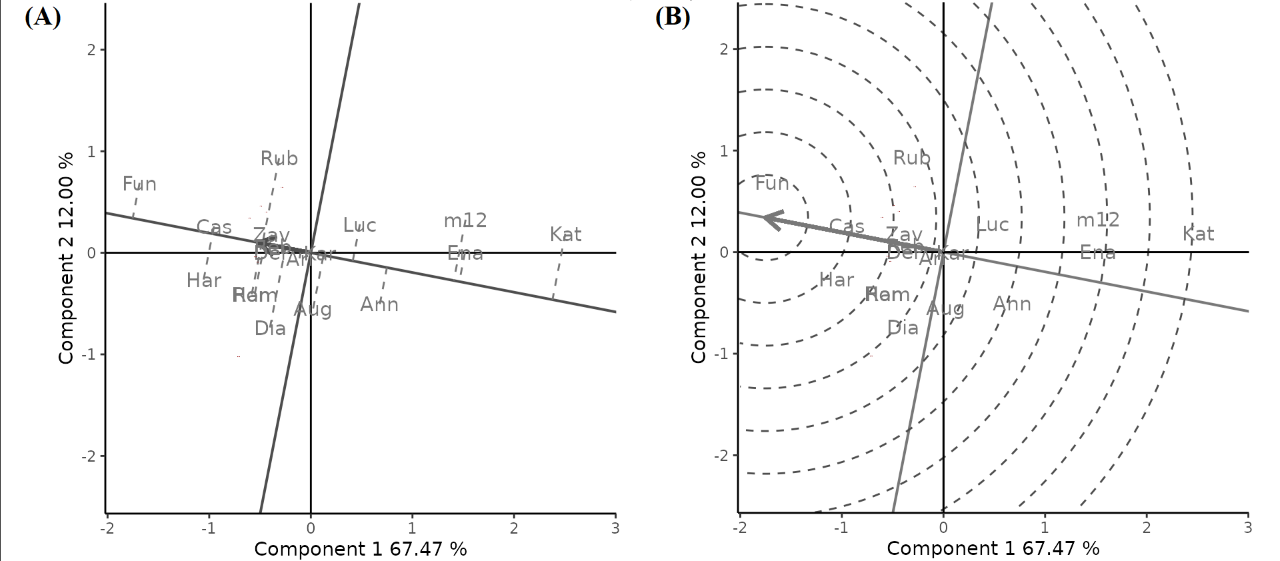
\includegraphics[width=0.90\textwidth]{./Graficos/MeanvsStability3.png}
	\end{center}
	\caption{(A) Evaluación de los cultivares con base en el rendimiento promedio y la estabilidad, y (B) clasificación de genotipos con respecto al genotipo ideal, basado en el método de partición de la descomposición en valores singulares enfocado en los genotipos.}
	\label{fig:evaluacionG}
\end{figure}
\end{tcolorbox}


\textbf{Evaluación de los ambientes con GGE biplot}

A pesar de que el objetivo principal de los EMA es seleccionar cultivares también es posible evaluar los ambientes. Esto incluye varios aspectos: (i) evaluar si la región objetivo pertenece a uno o más mega-ambientes; (ii) identificar mejores entornos de prueba; (iii) detectar ambientes redundantes que no brindan información adicional sobre cultivares; y (iv) determinar los ambientes que se pueden utilizar para la selección indirecta. Para ello, se enfoca la partición de los valores singulares en los ambientes al ajustar el modelo SREG (\emph{SVP = ``column"} en la función \textcolor{fandango}{GGEmodel()}). 

En la figura \ref{fig:evaluacionE} los ambientes están conectados con el origen de coordenadas a través de vectores, permitiendo comprender las interrelaciones entre ellos.  Esta visualización del biplot GGE se obtiene indicando \emph{Relationship Among Environments} (Figura \ref{fig:evaluacionE} (A)) en el parámetro \emph{type}. El coeficiente de correlación entre dos ambientes es aproximadamente el coseno del ángulo entre sus vectores. 
En este ejemplo se considera la relación entre los ambientes de ME1. El ángulo entre los vectores para los entornos NN93 y WP93 es de aproximadamente $10^{\circ}$ entre sus vectores; por lo tanto, están estrechamente relacionados; mientras que RN93 y OA93 presentan una correlación negativa débil ya que el ángulo es levemente mayor a $90^{\circ}$. El coseno de los ángulos no se traduce precisamente en coeficientes de correlación, ya que el biplot no explica toda la variabilidad en el conjunto de datos. Sin embargo, son lo suficientemente informativos como para comprender la interrelación entre los entornos de prueba. 

Si algunos de los ambientes tienen ángulos pequeños entre sí y, por lo tanto, están altamente correlacionados, la información sobre los genotipos obtenidos de estos ambientes debe ser similar. Si esta similitud se repite a través de los años, estos ambientes son redundantes y la evaluación de uno solo debería ser suficiente, permitiendo reducir costos en la experimentación.


La capacidad de discriminación así como la representatividad respecto del ambiente objetivo, son medidas fundamentales para un ambiente. Si no tiene capacidad de discriminación, no proporciona información sobre los cultivares y, por lo tanto, carece de utilidad. A su vez, si no es representativo no sólo que carece de utilidad sino que también puede proporcionar información sesgada sobre los cultivares evaluados. Para visualizar estas medidas, se define una coordenada ambiental promedio (AEC mencionado anteriormente) y el ambiente ideal como el centro de un conjunto de círculos concéntricos (Figura \ref{fig:evaluacionE} (B)). Para obtener este biplot se debe indicar \emph{Ranking Environments} en el argumento \emph{type} de \textcolor{fandango}{GGEPlot()}. El ángulo entre el vector de un ambiente y el eje proporciona una medida de la representatividad. Por lo tanto, EA93 e ID93 son los más representativos, mientras que RN93 y BH93 son los menos representativos del ambiente promedio, cuando se analiza ME1. Por otro lado, para ser discriminativo debe estar cercano al ambiente ideal. HW93 es el ambiente más cercano al ideal y, por lo tanto, es el más deseable del ME1, seguido por EA93 e ID93. Por el contrario, RN93 y BH93 fueron los ambientes de prueba menos deseables de ME1.  \\

\begin{tcolorbox}[skin=bicolor,
    colframe=aurometalsaurus,colback=backcolour,colbacklower=white,
    width=1\linewidth,
    height=0.89\linewidth,
    boxsep=-3mm]
\begin{lstlisting}
# Modelo SREG enfocando SVD en los ambientes
GGE_Epartition <- GGEmodel(ME1, genotype=``gen", environment=``env", response=``yield", SVP=``column")

# Relacion entre ambientes
GGEPlot(GGE_Epartition, type = ``Relationship Among Environments", footnote = F, titles = F)

# Clasificacion de ambientes con respecto al ambiente ideal
GGEPlot(GGE_Epartition, type = ``Ranking Environments", footnote = F, titles = F)
\end{lstlisting}
\tcblower\vskip-\baselineskip
\tcblower
\begin{figure}[H]
	\begin{center}
		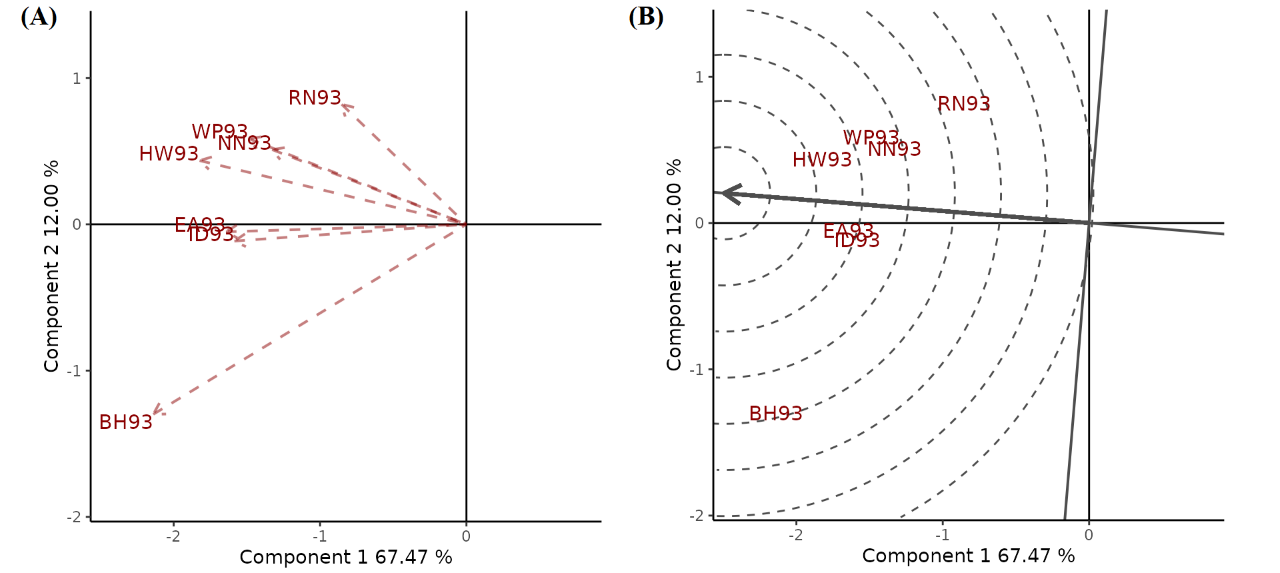
\includegraphics[width=0.90\textwidth]{./Graficos/RelationshipAmongEnvironments2.png}
	\end{center}
	\caption{(A) Relación entre ambientes y (B) clasificación de ambientes con respecto al ambiente ideal, basado en el escalado centrado en los genotipos.}
	\label{fig:evaluacionE}
\end{figure}
\end{tcolorbox}


\subsection{Uso del paquete para imputar matrices de datos incompletas}
\label{subsec:metimp}

Una limitación importante de los modelos presentados anteriormente es que requieren que el conjunto de datos este completo, es decir que todos los genotipos sean evaluados en todos los ambientes. Por lo tanto, en el paquete se incluyen una serie de metodologías de imputación desarrolladas específicamente para datos genotipo-ambiente recientemente publicadas, algunas de las cuales no se encuentran disponible en R, para superar el problema de las observaciones perdidas. Entre los métodos incluidos se encuentran: ``EM-AMMI", ``EM-SVD", ``Gabriel",``WGabiel''  y ``EM-PCA", los cuales se indican en la opción \emph{type} de la función \textcolor{fandango}{imputation()}. El formato requerido para el conjunto de datos de entrada es análogo al indicado en las otras funciones incluidas en el paquete. 

Para presentar un ejemplo, se eliminan algunas observaciones del conjunto de datos \emph{yan.winterwheat} ya que contaba con todos los registros completos:

\begin{tcolorbox}[skin=bicolor,
    colframe=aurometalsaurus,colback=backcolour,colbacklower=white,
    width=1\linewidth,
    height=0.15\linewidth,
    boxsep=-3mm]
\begin{lstlisting}
# Generando datos faltantes
yan.winterwheat [1,3] <- NA
yan.winterwheat [3,3] <- NA
yan.winterwheat [2,3] <- NA
\end{lstlisting}
\end{tcolorbox}

La imputación de valores perdidos con el método ``EM-AMMI" se puede realizar de la siguiente manera:

\begin{tcolorbox}[skin=bicolor,
    colframe=aurometalsaurus,colback=backcolour,colbacklower=white,
    width=1\linewidth,
    height=0.08\linewidth,
    boxsep=-3mm]
\begin{lstlisting}
imputation(yanwinterwheat, PC.nb = 2, genotype = ``gen", environment = ``env", response = ``yield", type = ``EM-AMMI")
\end{lstlisting}
\end{tcolorbox}

El resultado es la matriz con datos imputados en aquellas celdas vacías. 

\section{Aplicación web \emph{Geneticae}}

Siguiendo el procedimiento descripto se desarrolló la aplicación web \emph{Geneticae}, con el objetivo de proporcionar una interfaz gráfica de usuario para el paquete, de modo que pueda ser utilizado por fitomejoradores y analistas sin experiencia previa en programación R. 

Es un software interactivo, no comercial y de código abierto, que ofrece una alternativa gratuita al software comercial disponible para analizar datos provenientes de ensayos multiambientales. Momentáneamente se encuentra disponible en un servidor gratuito con una cuota mensual de horas de uso, al cual se puede acceder con el enlace \url{https://geneticae.shinyapps.io/geneticae-shiny-web-app/} o desde la página web \url{https://www.cefobi-conicet.gov.ar/bases-de-datos-y-programas/} del Centro de Estudios Fotosintéticos y Bioquímicos del Consejo Nacional de Investigaciones Científicas y Técnicas (CONICET).

A la brevedad la aplicación estará disponible para su uso ilimitado en los servidores del Centro de Cómputos de Alto Rendimiento situado en el Datacenter del Centro Científico Teconológico (CCT) de CONICET Rosario.  Como parte de este trabajo se solicitó al Centro de Cómputos la instalación de un \emph{Shiny Server}  (software que permite publicar este tipo de aplicaciones), habiendo resultado exitosa la publicación de una primera versión de prueba de \emph{Geneticae}. Actualmente, la versión final se encuentra en la cola de trabajo del equipo del CCT para su instalación definitiva y consiguiente apertura al público general.

En las subsecciones siguientes se presentará un ejemplo de cómo cargar y analizar datos con la aplicación web \emph{Geneticae}.

\subsection{Lectura de un archivo de datos para el uso de la aplicación web \emph{Geneticae}}

La aplicación web \emph{Geneticae} requiere que los datos de entrada se encuentren en archivos de texto plano, con delimitaciones por comas o punto y coma (formato .csv) o tabulaciones (formato .txt). Los nombres de las columnas pueden ubicarse en la primera fila del archivo (\emph{heading}). Los datos deben estar en formato largo, es decir, cada fila debe corresponder a una observación y cada columna a una variable (genotipo, ambiente, fenotipo observado y, si existe, repetición). Si cada genotipo ha sido evaluado más de una vez en cada ambiente, la media fenotípica requerida por el modelo SREG y AMMI para cada combinación de genotipo y ambiente se calcula internamente antes de ajustar dichos modelos. Las variables adicionales que no se utilizarán en el análisis pueden estar presentes en el conjunto de datos. No se permiten valores perdidos.

Los dos conjuntos de datos \emph{plrv} y \emph{yanwinterwheat} descriptos en la subsección \ref{subsec:datosejemplos} están disponibles en la pestaña \emph{Data $\rightarrow$ Example datasets} y se pueden descargar en formato .csv (Figura \ref{fig:dataexample}) para poder seguir el tutorial de uso de la aplicación. El conjunto de datos \emph{yanwinterwheat} no tiene repeticiones, mientras que \emph{plrv} sí. 

\begin{figure}[H]
	\begin{center}
		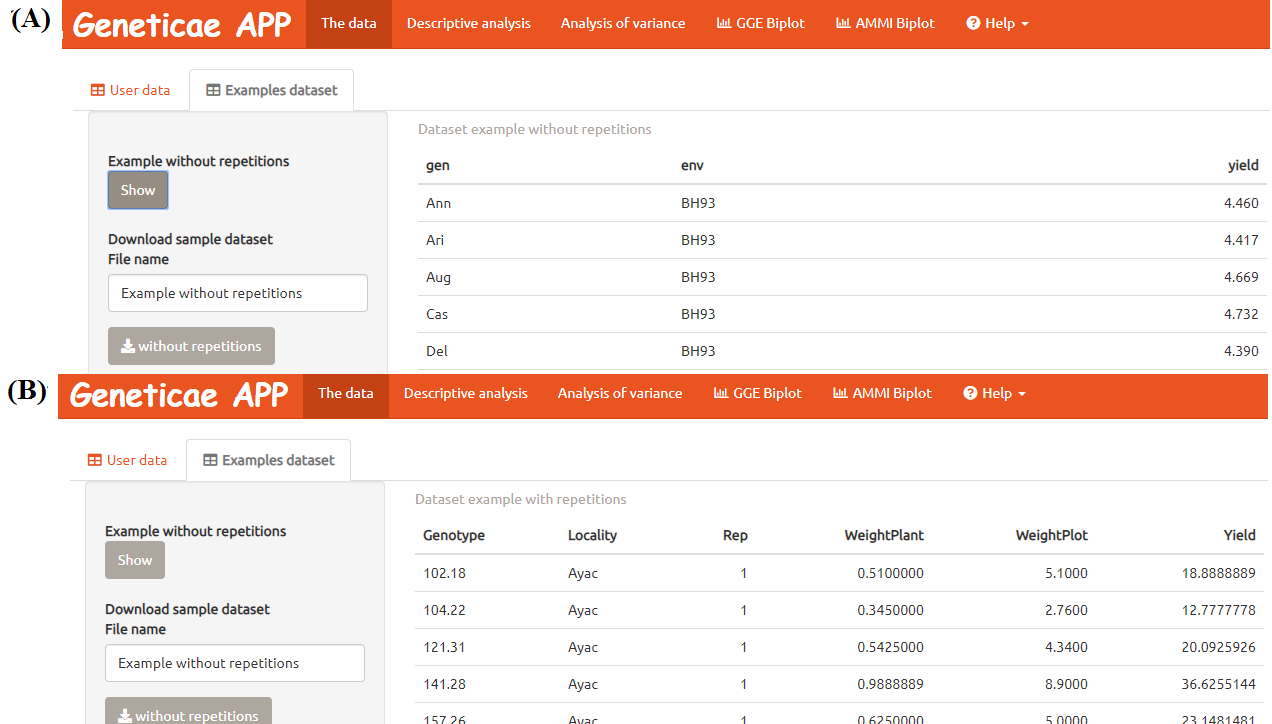
\includegraphics[width=0.60\textwidth]{./Graficos/www/exampledata2.png}
	\end{center}
	\caption{Conjuntos de datos (A) \emph{plrv} y (B) \emph{yanwinterwheat} disponibles en la aplicación web \emph{Geneticae}.}
	\label{fig:dataexample}
\end{figure}

En los siguientes ejemplos se trabajará con \emph{yanwinterwheat} para mostrar el uso de la aplicación. Luego de obtener el archivo de datos con el formato indicado, es posible importarlo en la pestaña \emph{Data $\rightarrow$ Upload data}. Por ejemplo, para importar \emph{yanwinterwheat}, se debe cargar el archivo .csv. Una vez cargado, se debe indicar que está delimitado por comas, que en la primera fila contiene los nombres de cada variable (\emph{heading}) y los nombres de las columnas en las cuales se encuentra la información del genotipo, ambiente y rasgo fenotípico (\emph{gen}, \emph{env} y \emph{yield} en este ejemplo) (Figura \ref{fig:fig431}). Si hay repeticiones disponibles, se debe especificar el nombre de la columna con dicha información; de lo contrario, el campo queda vacío. 

 \begin{figure}[h]
	\begin{center}
		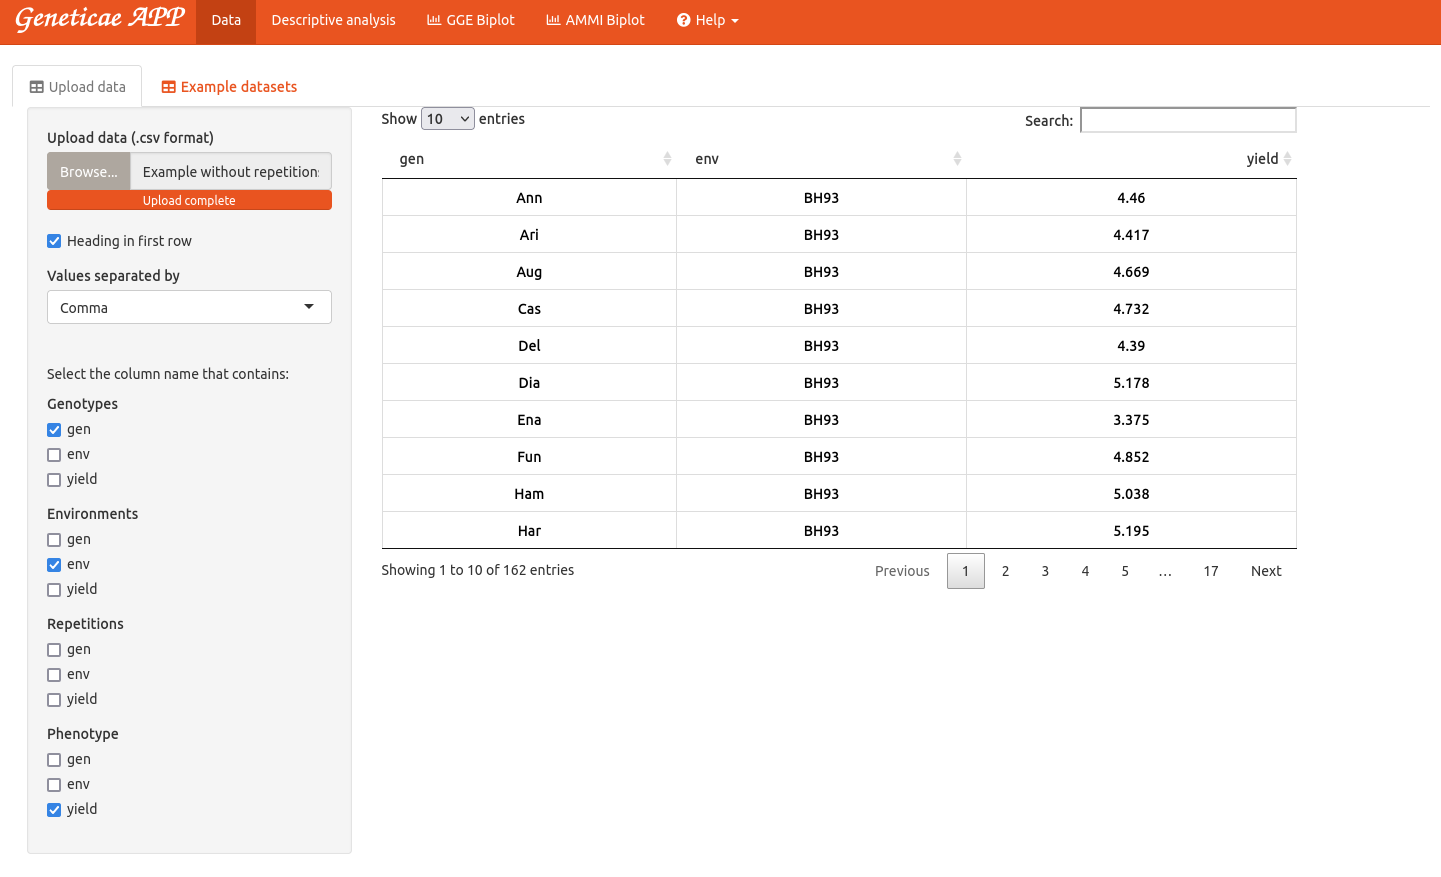
\includegraphics[width=0.65\textwidth]{./Graficos/www/Data.png}
	\end{center}
	\caption{Importar el conjunto de datos \emph{yanwinterwheat} en la aplicación web \emph{Geneticae}.}
	\label{fig:fig431}
\end{figure}

\hspace{1cm}

\subsection{Uso de la aplicación web \emph{Geneticae} para análisis descriptivo}

Cualquier estudio debe comenzar con un análisis descriptivo del conjunto de datos. La pestaña \emph{Descriptive Analysis} proporciona algunas herramientas para esto, como  \emph{boxplot}, diagrama y matriz de correlación y gráficos de interacción.

Un \emph{boxplot} que compara el rasgo cuantitativo entre ambientes o genotipos puede ser de interés (Figura \ref{fig:figdesc1}). Las medidas de resumen utilizadas para su construcción se muestran de forma interactiva moviendo el \emph{mouse} dentro del panel de la figura. Además, se puede descargar en formato .png o como un archivo interactivo .HTML, haciendo clic en la cámara que aparece en el gráfico o en el botón Descargar, respectivamente. El usuario puede personalizar algunos aspectos del gráfico, como el color de las cajas y los nombres de los ejes. 

\begin{figure}[h]
	\begin{center}
		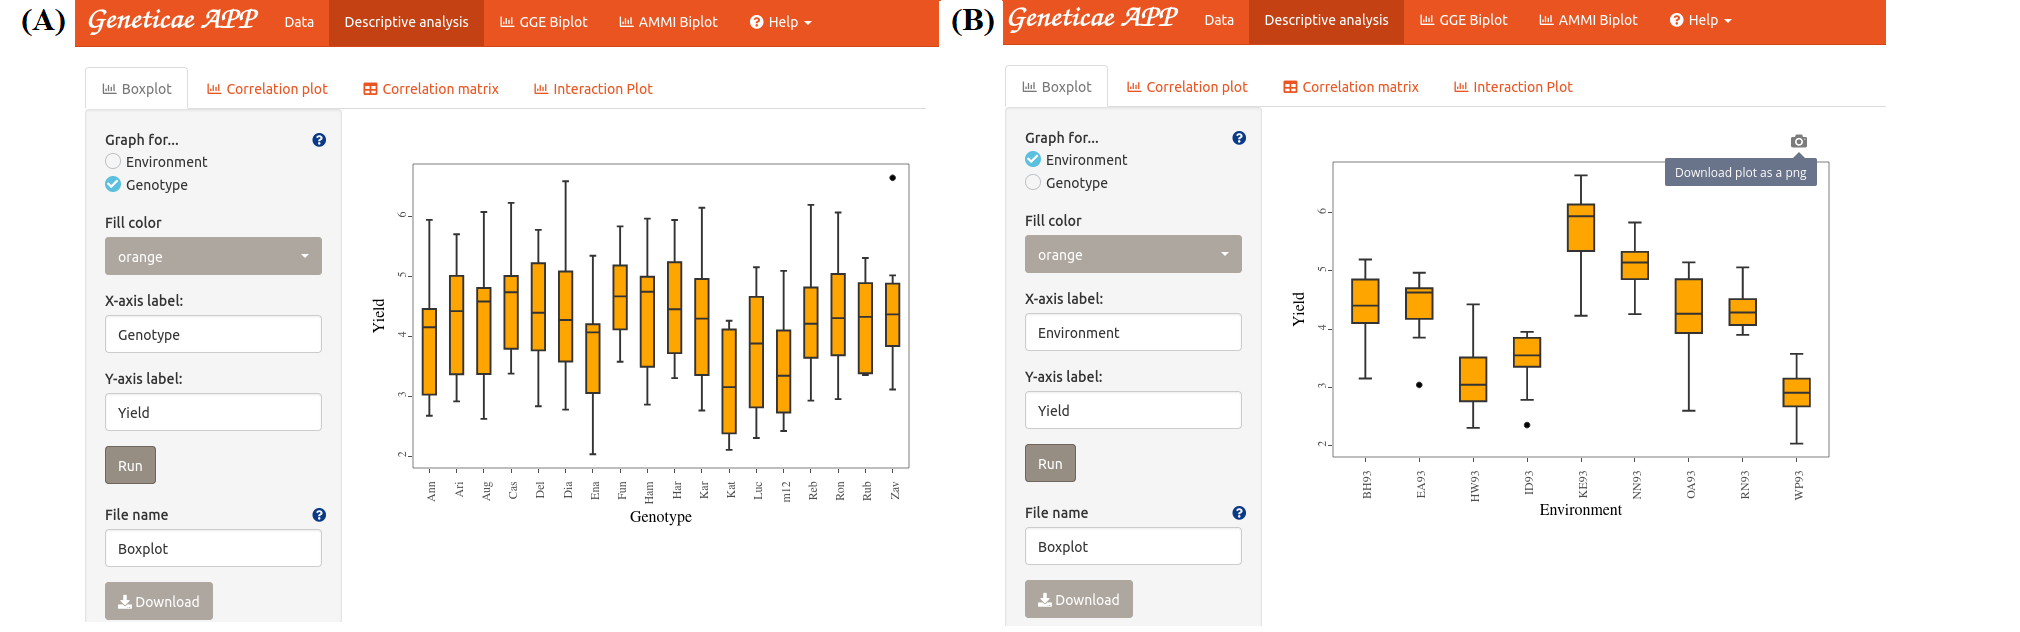
\includegraphics[width=0.9\textwidth]{./Graficos/www/boxplot.png}
	\end{center}
	\caption{Diagrama de caja de (A) genotipos y (B) ambientes para el conjunto de datos \emph{yanwinterwheat} obtenido con la aplicación web \emph{Geneticae}.}
	\label{fig:figdesc1}
\end{figure}

Los coeficientes de correlación de Pearson o Spearman entre genotipos se pueden mostrar con un gráfico o una matriz (Figura \ref{fig:figdesc2}). Gráficamente, las correlaciones positivas se muestran en azul y las negativas en rojo, mientras que la intensidad del color y el tamaño del círculo son proporcionales a la magnitud de los coeficientes de correlación. La gráfica de correlación se puede descargar en formato .png. En el ejemplo, se observan altas correlaciones entre el rendimiento de los genotipos estudiados. 

\begin{figure}[h]
	\begin{center}
		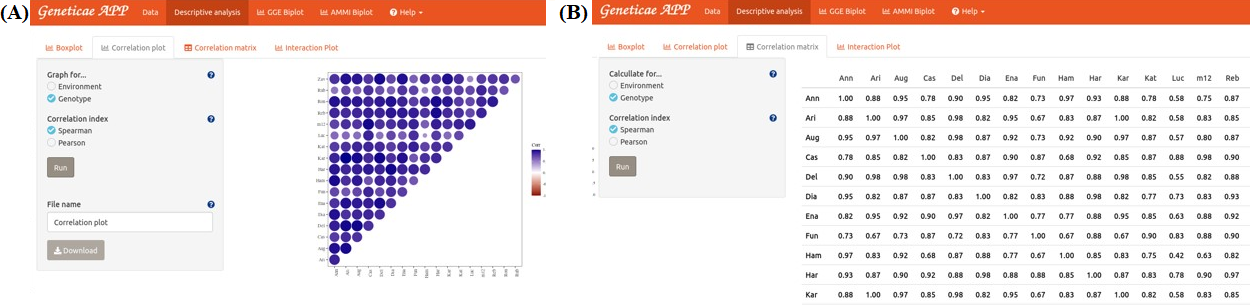
\includegraphics[width=0.9\textwidth]{./Graficos/www/correlacion.png}
	\end{center}
	\caption{(A) Gráfico y (B) matriz de correlación entre genotipos para el conjunto de datos \emph{yanwinterwheat} obtenido con la aplicación web \emph{Geneticae}.}
	\label{fig:figdesc2}
\end{figure}


Dado que la IGA genera respuestas genotípicas diferenciales en diferentes ambientes complicando la selección de los mejores cultivares, una gráfico de interacción puede ser de interés (Figura \ref{fig:figdesc3}). El cambio en el efecto genotípico a través de los ambientes se muestra en la figura \ref{fig:figdesc3} A, mientras que el cambio en el efecto ambiental a través de los genotipos en la figura \ref{fig:figdesc3} B. Estos también son gráficos interactivos por lo que es posible descargarla en formatos .HTML o .png con el botón Descargar o haciendo clic en la cámara que aparece en el gráfico, respectivamente. Además, el usuario puede personalizar los nombres de los ejes. En este ejemplo se pueden ver inconsistencias en el desempeño de genotipos en diferentes ambientes. 


\begin{figure}[H]
	\begin{center}
		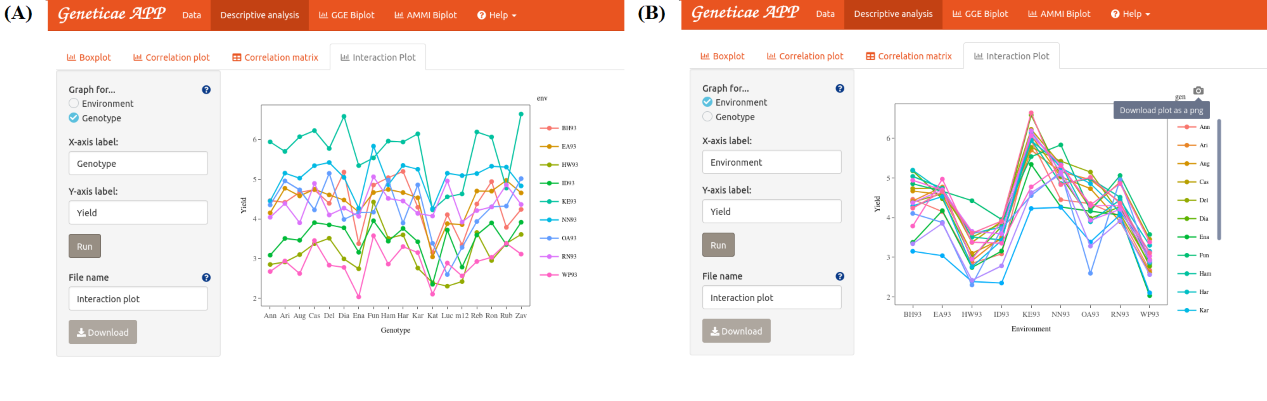
\includegraphics[width=0.9\textwidth]{./Graficos/www/interaction.png}
	\end{center}
	\caption{Gráfico de interacción para (A) ambientes a través de genotipos y (B) genotipos a través de los ambientes para conjunto de datos de \emph{yanwinterwheat} obtenido con la aplicación web \emph{Geneticae}.}
	\label{fig:figdesc3}
\end{figure}


\subsection{Uso de la aplicación web \emph{Geneticae} para ajustar el modelo SREG}

La aplicación web \emph{Geneticae} permite generar las vistas del biplot GGE presentados en la subsección \ref{subsec:SREGpaquete} mediante la pestaña \emph{GGE Biplot}. Del mismo modo que en el paquete \emph{geneticae}, los cultivares se presentan en minúsculas y los ambientes en mayúsculas. Dado que el modelo SREG requiere una única observación para cada combinación de genotipo y ambiente, si hay repeticiones, el valor fenotípico promedio se calcula automáticamente antes de ajustar el modelo. No se permiten valores perdidos. 

Se debe seleccionar el método de partición de los valores singulares (\emph{SVP type}). Como se mencionó anteriormente esta elección no altera las relaciones o interacciones relativas entre genotipos y ambientes, aunque la apariencia del biplot será diferente (Yan, 2002). La opción simétrica permite la comparación tanto de genotipos como de ambientes (opción por defecto); \emph{Genotype-Focused} muestra la interrelación entre genotipos con mayor precisión que cualquier otro método y \emph{Environment-Focused} es la que más informa sobre las interrelaciones entre ambientes. Una nota a pie del gráfico indica el método de centrado utilizado (para el biplot GGE siempre es \emph{tester-center}), el método SVP elegido por el usuario y que no se aplica ninguna escala a los datos. Además, se puede agregar el porcentaje de variabilidad de G e IGA explicado por las dos PC, mientras que la inclusión de títulos, ejes y etiquetas es opcional. Ciertos atributos estilísticos de dichos gráficos se pueden personalizar como el color y tamaño de los identificadores de los genotipos y de los ambientes. Los gráficos pueden ser descargados.  

El biplot básico, la vista del biplot GGE que muestra los cultivares más adecuados para un ambiente particular (OA93), los ambientes más adecuados para un genotipo (Kat), la comparación de dos genotipos (Cas y Kat) y la vista del poligono se pueden obtener como se indica en la figura \ref{fig:ggebip1}, donde el escalado es el simétrico (\emph{SVP type $\rightarrow$ symmetrical}) y las opciones de \emph{plot type} son \emph{Biplot,
Selected Environment, Selected Genotype, Comparison of Genotype} y \emph{Which Won Where/What}, respectivamente. Al indicar \emph{Selected Environment} el ambiente de interés se debe especificar, de igual modo cuando se utiliza \emph{Selected Genotype} y 
\emph{Comparison of Genotype} se debe señalar cuál es el genotipo a analizar.

\begin{figure}[H]
	\begin{center}
		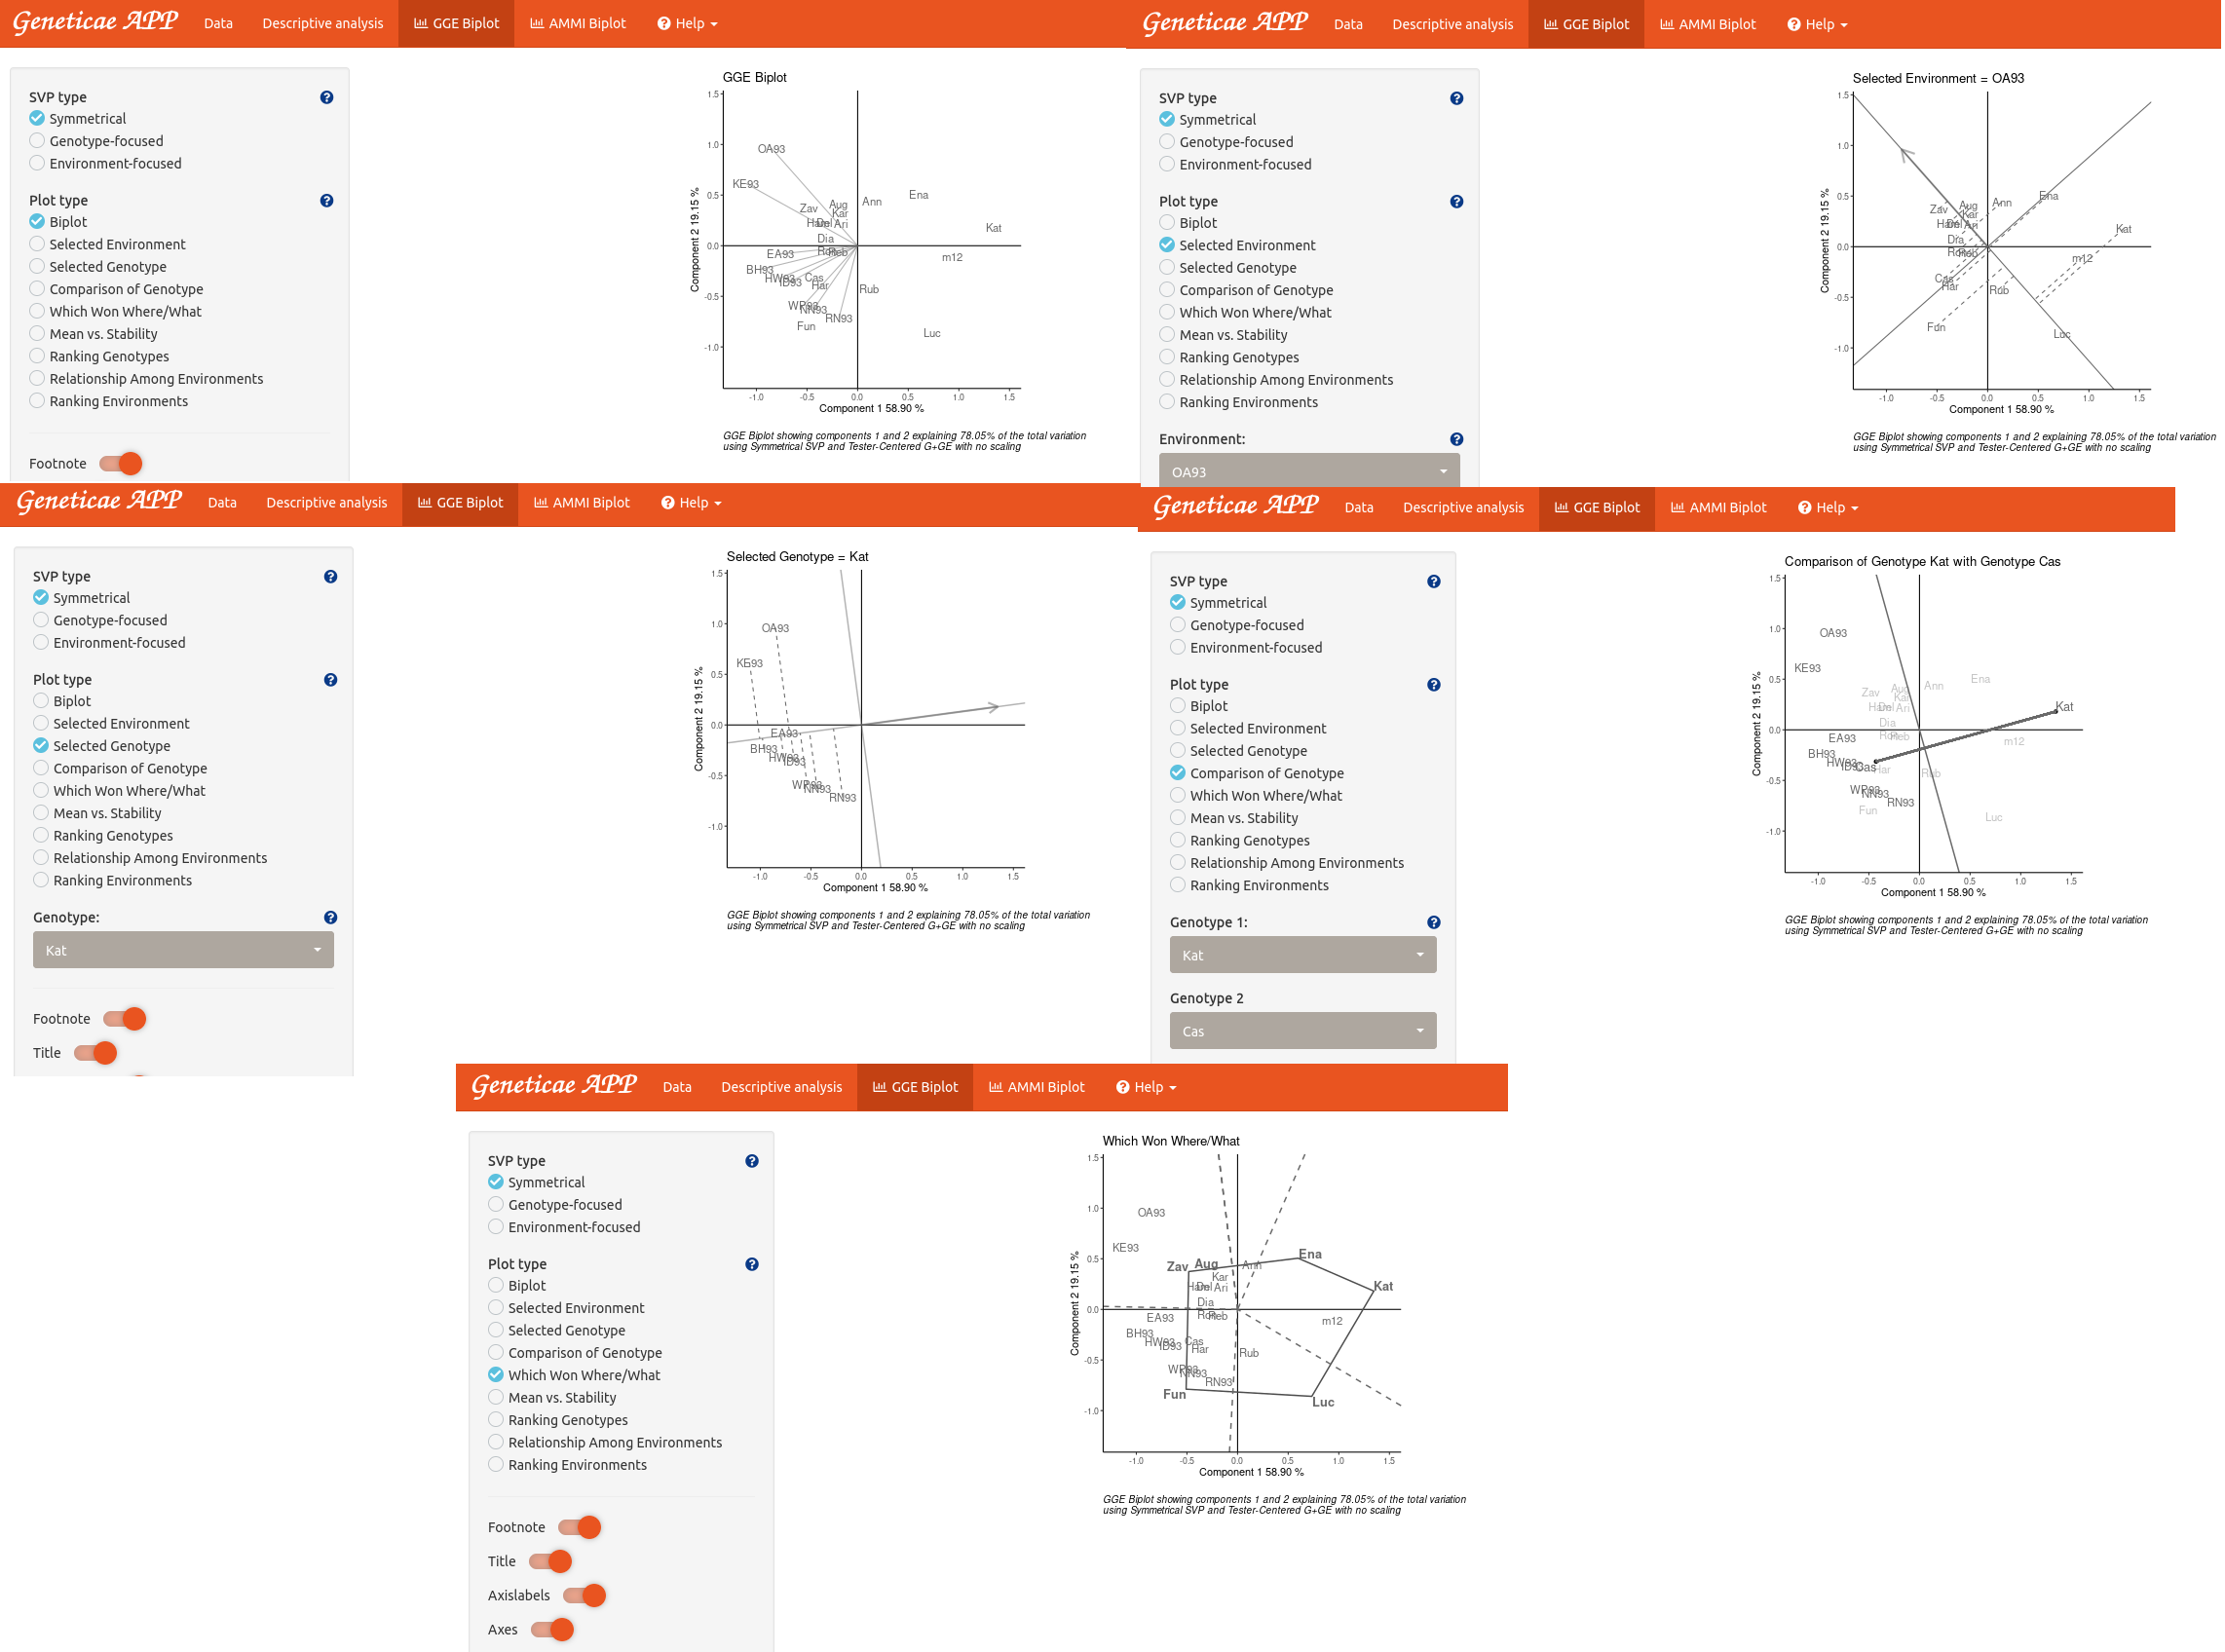
\includegraphics[width=0.9\textwidth]{./Graficos/www/GGE_biplotAPP1.png}
	\end{center}
	\caption{Vistas del biplot GGE usando la partición en valores singulares simétrica obtenidos con la aplicación web \emph{Geneticae}.}
	\label{fig:ggebip1}
\end{figure}

La selección de cultivares dentro de cada mega-ambiente se realiza con la partición de valores singulares enfocada en los genotypos (\emph{SVP type $\rightarrow$ genotype-focused}), y los tipos de gráficos que se pueden realizar son: \emph{Mean vs. Stability} que permite la visualización de la media y estabilidad de genotipos y \emph{Ranking Genotypes} que compara las cultivares con el ``ideal" (Figura \ref{fig:ggebip2}). Dado que estos análisis son propios de cada mega-ambiente, al indicar alguno de estas vistas del biplot GGE se tendrá que señalar cuales son los ambientes que forman el mega-ambiente de interés. 


\begin{figure}[h]
	\begin{center}
		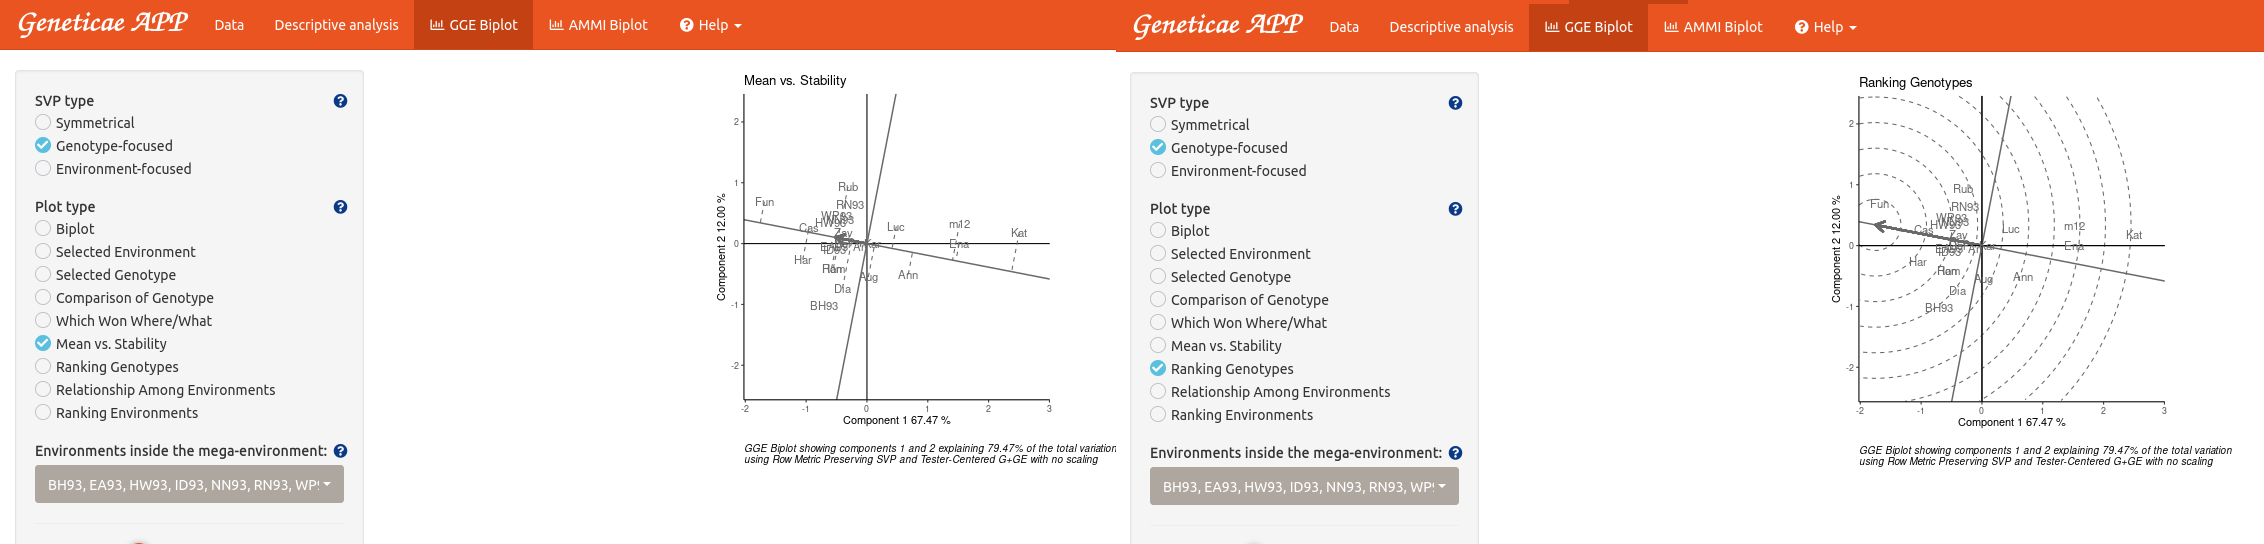
\includegraphics[width=0.95\textwidth]{./Graficos/www/GGE_biplotAPP2.png}
	\end{center}
	\caption{Vistas del biplot GGE usando la partición de valores singulares enfocada en los genotipos obtenidos con la aplicación web \emph{Geneticae}.}
	\label{fig:ggebip2}
\end{figure}

Por último, para el análisis de los ambientes de cada mega-ambiente se utiliza el método de partición de valores singulares centrado en los ambientes (\emph{SVP type $\rightarrow$ environment-focused}). El tipo de gráfico \emph{Relationship Among Environments} permite comprender la interrelación entre los ambientes, mientras que \emph{Ranking Environments} se utiliza para visualizar la capacidad de discriminación y representatividad (Figura \ref{fig:ggebip3}). Como en el caso anterior, al indicar alguna de estas vistas del biplot GGE se tendrá que señalar cuales son los ambientes que forman el mega-ambiente de interés. 


\begin{figure}[h]
	\begin{center}
		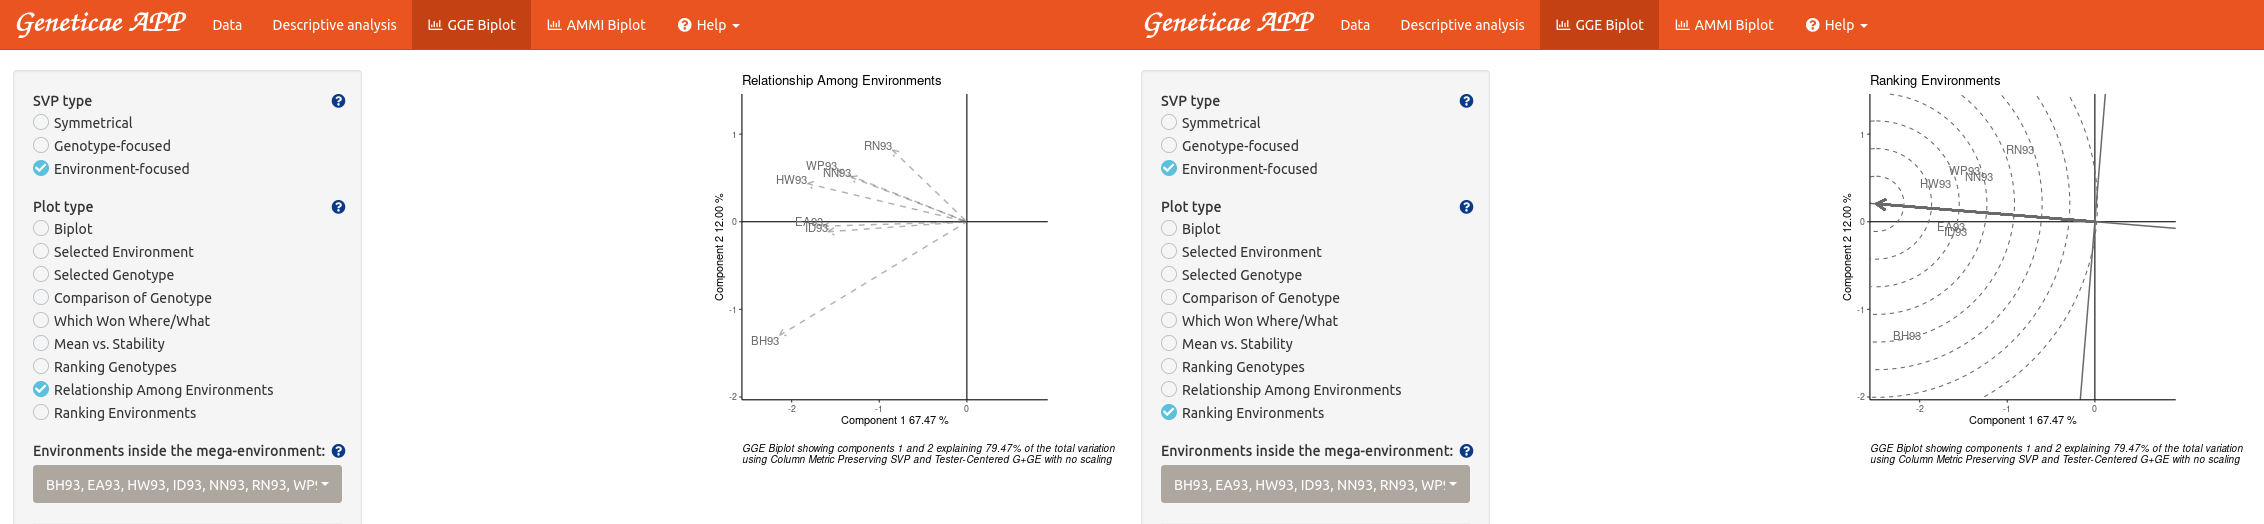
\includegraphics[width=0.95\textwidth]{./Graficos/www/GGE_biplotAPP3.png}
	\end{center}
	\caption{Vistas del biplot GGE usando la partición de valores singulares enfocada en los ambientes obtenidas con la aplicación web \emph{Geneticae}.}
	\label{fig:ggebip3}
\end{figure}


\subsection{Uso de la aplicación web \emph{Geneticae} para ajustar el modelo AMMI}

La pestaña \emph{AMMI Biplot} crea el biplot GE. Dado que las alternativas clásica y robustas requieren una única observación para cada combinación de genotipo y ambiente, si hay repeticiones, el valor promedio fenotípico se calcula automáticamente antes de ajustar el modelo. No se permiten valores perdidos. Como con las figuras anteriores, se ofrecen opciones de configuración y de descarga.

Por ejemplo, para obtener el biplot GE derivado del modelo AMMI clásico se debe indicar AMMI en \emph{plot type} (Figura \ref{fig:figammiapp}). En caso de contar con \emph{outliers}, alguna de las alternativas robustas (rAMMI, hAMMI, gAMMI, lAMMI o ppAMMI).
 

\begin{figure}[h]
	\begin{center}
		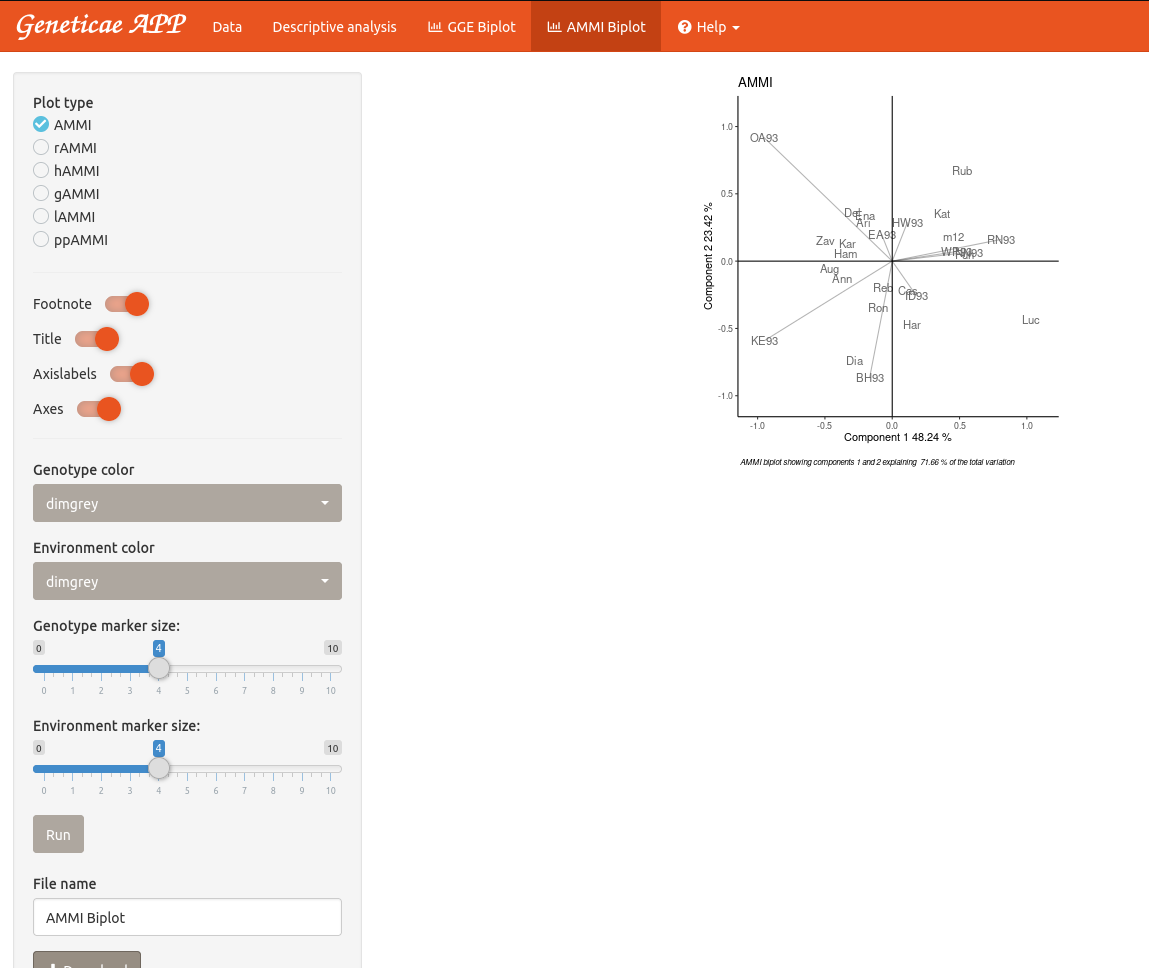
\includegraphics[width=0.70\textwidth]{./Graficos/AMMI_GE.png}
	\end{center}
	\caption{Biplot GE derivado del modelo AMMI clásico basado en datos de rendimiento de trigo de invierno obtenido de Ontario en 1993 obtenido con la aplicación web \emph{Geneticae}.}
	\label{fig:figammiapp}
\end{figure}


\subsection{Ayuda}

En la pestaña \emph{Help} se presenta información general, un tutorial y un video sobre cómo utilizar la aplicación web \emph{Geneticae}.
